\newpage
\section{Comparación}
\par En esta sección del informe se compararán las implementaciones de los diferentes algoritmos en ASM contra los algoritmos en C, compilados con distintas
opciones de optimización (O0, O1, O2, O3).
\par Todos los algoritmos a continuación tienen una diferencia fundamental con su contraparte en C, que es la utilización de técnicas de procesamiento vectorial.
Por esto era esperable ver una mejoría en el rendimiento de los mismos, como se muestra en los siguientes gráficos. \\

\begin{figure*}[h]
    \centering
        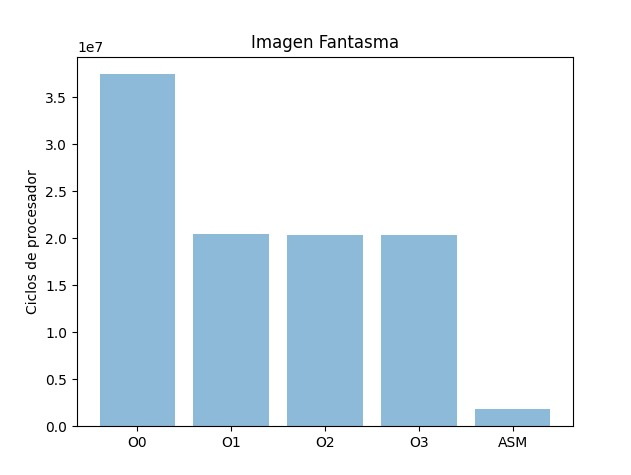
\includegraphics[width=0.5\linewidth]{img/ImagenFantasma.jpeg}\hfil
        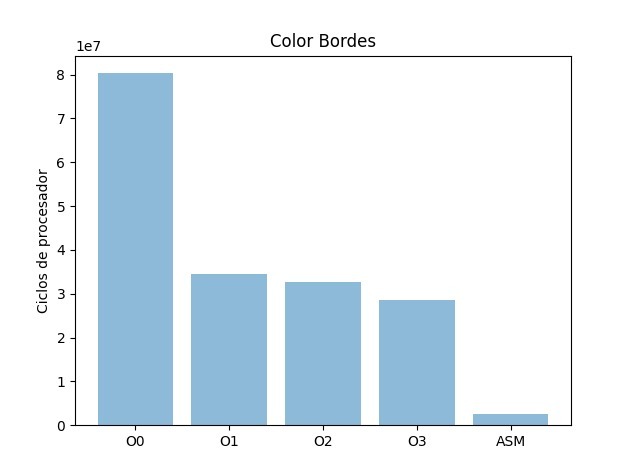
\includegraphics[width=0.5\linewidth]{img/ColorBordes.jpeg}\par\medskip
        \caption{Comparación de promedio de rendimiento para Imagen Fantasma entre ASM y distintas optimizaciones de C}
        \caption{Comparación de promedio de rendimiento para Color Bordes entre ASM y distintas optimizaciones de C}
    \end{figure*}
    
    \begin{figure*}[h]
    \centering
    \begin{tabular}{cc}
        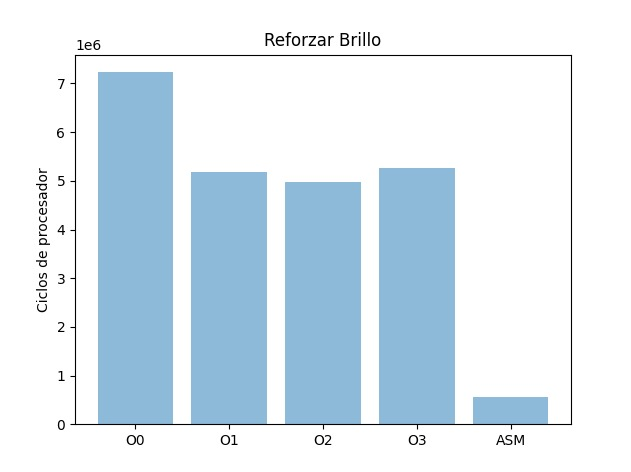
\includegraphics[width=0.5\linewidth]{img/ReforzarBrillo.jpeg}&
    \end{tabular}
    \caption{Comparación de promedio de rendimiento para Reforzar Brillo entre ASM y distintas optimizaciones de C}
\end{figure*}

\par Estas últimas figuras miden el promedio de ciclos de código, donde se excluyeron de la población muestral todas aquellas muestras que se encuentren 2 veces por encima de la desviación estándar.
Estas mediciones fueron hechas con una amplia variedad de imágenes de distintos tamaños y como se puede apreciar, la diferencia de rendimiento entre las implementaciones en ASM es superior
a cualquier optimización de C.

\par Al usar imágenes de distintos tamaños para medir el rendimiento, surgió la pregunta de si el mismo afectaba a la performance de los algoritmos (relativa entre estos), tanto en C como en ASM.
Para esto se escogió un subconjunto de estas imágenes, las cuales fueron reconvertidas para tener los siguientes tamaños: 128x64, 256x128, 512x256 y 1024x512.


\begin{figure*}[h]
    \centering
        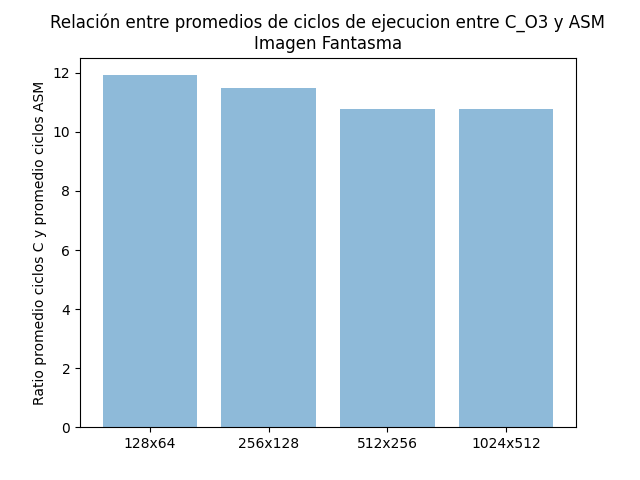
\includegraphics[width=0.5\linewidth]{img/RelacionASMCImagenFantasma.png}\hfil
        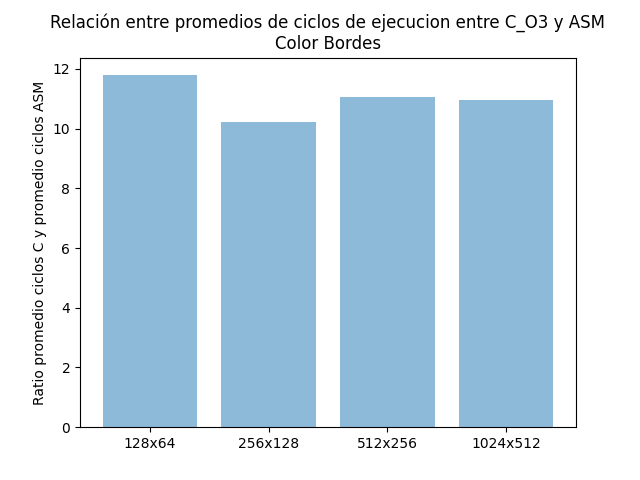
\includegraphics[width=0.5\linewidth]{img/RelacionASMCColorBordes.png}\par\medskip
        \caption{Ratio entre promedios de rendimiento para Imagen Fantasma entre ASM y C_O3 con distintos tamaños de imagenes}
        \caption{Ratio entre promedios de rendimiento para Color Bordes entre ASM y C_O3 con distintos tamaños de imagenes}
    \end{figure*}
    
    \begin{figure*}[h]
    \centering
    \begin{tabular}{cc}
        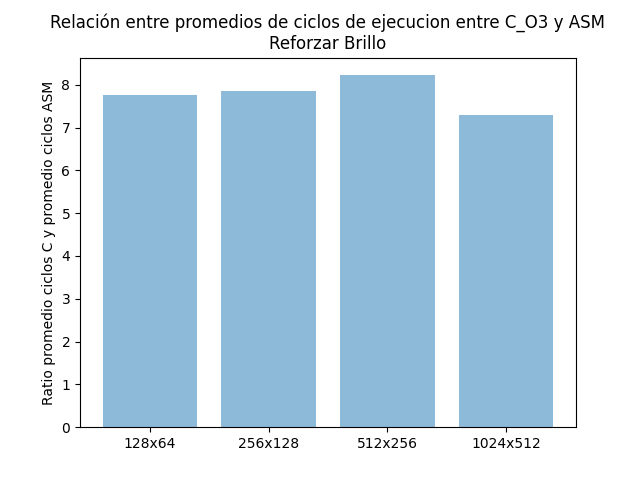
\includegraphics[width=0.5\linewidth]{img/RelacionASMCReforzarBrillo.png}&
    \end{tabular}
    \caption{Ratio entre promedios de rendimiento para Reforzar Brillo entre ASM y C_O3 con distintos tamaños de imagenes}
\end{figure*}
\par Utilizando el mismo método de cálculo de promedios con este nuevo conjunto de imágenes se ve que se mantiene constante el ratio de ciclos en C / ciclos en ASM, lo cual asegura que llevar a cabo 
la comparación ASM vs. C utilizando distintos tamaños de imagen no afecta qué implementación resulta ser la mejor.